  \item Zarządzanie dostawą\\
  
  Opis słowny - na wniosek klienta, lub z powodu decyzji sklepu, zamówione
  dowary mogą być dostarczone różnymi środkami transportu. Ta opcja umożliwia
  ingerencję w dane zapisane podczas składania zamówienia.
  
    \begin{longtable}{|p{5cm}|p{7cm}|}
 	\hline
	\textbf{Aktor} & Pracownik \\
	\hline
	\textbf{Warunki początkowe} & Pracownik zalogowany, zmiany wprowadzane na
	wniosek klienta
	\\
	\hline
	\textbf{Opis przebiegu interakcji} & Wybór zarządzania zamówieniami,
	z listy zamówień zaznaczenie konkretnego, opcja Edycji Dostawy
	\\
	\hline
	\textbf{Sytuacje wyjątkowe} & Brak żądanego zamówienia
	\\
	\hline
	\textbf{Warunki końcowe} & Aktualizacja danych dotyczących zamówienia
	\\
	\hline
 \end{longtable}
  
  
  \begin{tabularx}{\linewidth}{c X}
  Aktor: & Pracownik \\
  Opis: & Termin realizacji zamówienia oraz sposób dostawy mogą być
  modyfikowany dowolnie w zależności od możliwości biznesowych Sklepu i
  aktualnego stanu zamówienia.
  \end{tabularx}
	\begin{enumerate}
	  \item Z listy zamówień użytkownik wybiera jedno i wybiera opcję Edycji
	  Dostawy
	  \item System prezentuje informacje o wybranym sposobie i terminie dostawy
	  \item Użytkownik wybiera opcję Zmiany daty realizacji
	  \item System prezentuje widok kalendarza z zaznaczoną dotychczasową datą
	  realizacji.
	  \item Użytkownik przesuwa datę realizacji projektu i ma możliwość podania
	  wiadomości wyjaśniającej modyfikację.
	  \item Użytkownik wybiera opcję Zmiany sposobu dostawy
	  \item System wyświetla wszystkie aktualnie dostępne opcje razem ze
	  szczegółami (cena, średni czas)
	  \item Użytkownik dokonuje wyboru środka transportu i zatwierdza zmiany
	  \item System aktualizuje koszt całego zamówienia uwzględniając kwotę
	  transportu oraz wysyła powiadomienie o zmianach (termin lub/i sposób dostawy)
	  do klienta wraz z informacją wyjaśniającą wpisaną przez pracownika.
	\end{enumerate}
	
	\begin{figure}[H]
    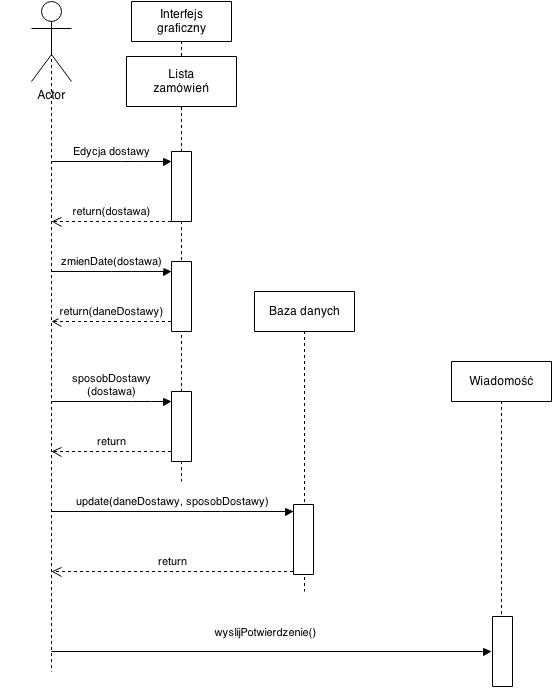
\includegraphics[width=\textwidth,
    height=0.5\textheight]{graphics/UseCase/Zamowienia/ZarzadzanieDostawaSD.png}
    \caption{Diagram sekwencji dla przypadku użycia Zarządzanie dostawą
    - scenariusz główny}
\end{figure}
	

  \item Ustawianie aktualnego stanu zamówienia\\
  \begin{tabularx}{\linewidth}{c X}
  Aktor: & Pracownik \\
  Opis: & Zamówienie może znajdować się w pewnych stanach realizacji (np. w
  przygotowaniu, w realizacji, wysłane - konkretne stany określają wymagania
  niefunkcjonalne). Istnieje możliwość zmiany aktualnego stanu zamówienia.
  \end{tabularx}
	\begin{enumerate}
	  \item Z listy zamówień pracownik wybiera jedno i wybiera opcję Zmień Stan
	  \item System prezentuje widok z dostępnymi stanami dla danego zamówienia
	  \item Pracownik dokonuje wyboru i zatwierdza zmiany.
	  \item Jeśli pracownik wybiera opcję Powiadom, to system powiadamia klienta o
	  zmianie stanu jaka nastąpiła i przesyła krótkie wyjaśnienie.
	\end{enumerate}
	 
